\subsection{Representation and Fusion Procedure}
The proposed system is inspired by\cite{Kolev2006} in that the representation used for the shape of the object to be modelled is a volume 
of probabilities, pertaining to posteriors over a voxels assignment to being either on the objects surface or not. In the proposed system this 
volume of posterior probabilities is `fused' into with each frame, much like the fusion process in systems such as KinectFusion\cite{Newcombe2011} 
and InfiniTAM\cite{Prisacariu2014}.

The probabilities that are `fused' into the volume are generated from an appearance model, initialised prior to reconstruction by a Maximum 
Likelihood procedure over the first frame of the RGB image. There are two appearance models, one for the foreground object and one for 
the background, with the foreground object indicated by a bounding box on the first RGB frame. A normal distribution is fitted over the colour 
features of each class, foreground and background. During the fusion process, the PDF's of these distributions are evaluated on the latest 
colour observation for a voxel and posterior's are computed and updated accordingly in the probability volume. Only those voxels with a 
posterior higher for the foreground are rendered.

\subsection{Probabilistic Formulation of Object Reconstruction}
As previously highlighted, central to the proposed system is a volume of posterior probabilities pertaining to a voxels membership of an object 
point versus a background scene point. This allows one to formulate the full joint distribution over the object as the following Probabilistic 
Graphical Model:-
\begin{figure}[h]
	\centering
	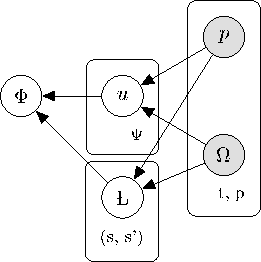
\includegraphics{graphical_models/pgm1.pdf}
\end{figure}
Where $\mathbf{\Phi}$ is the shape to be reconstructed, $\mathbf{u}$ is the appearance model volume, $\mathbf{L}$ is the 
set of consistency constraints for each adjacent sub volume pair, $\mathbf{\Omega}$ is the set of RGBD image pixels and $\mathbf{p}$ the 
set of poses over time.

This gives rise to the following analytical formulation of the above distribution:-

\begin{equation}
\begin{split}
P(\mathbf{\Phi}, \mathbf{\Omega}, \mathbf{p}, \mathbf{u}, \mathbf{L}) = 
\prod_{v \in \mathcal{V}}P(\mathbf{\Phi}|\mathbf{u}_{v}) 
\prod_{t=0}^{\infty}\prod_{p \in \mathcal{P}}\prod_{(s, s') \in \mathcal{S}}\\
P(\mathbf{u_{v}}|\mathbf{\Omega}_{p, t}, \mathbf{p}_{t}, \mathbf{L}_{(s, s')})
P(\mathbf{L}_{(s, s')}|\mathbf{\Omega}_{p, t}, \mathbf{p}_{t})\\
P(\mathbf{L}_{(s, s')})P(\mathbf{p}_{t})P(\mathbf{\Omega}_{p, t})
\end{split}
\end{equation}
Where $\mathcal{V}$ is the set of voxels across all sub volumes, $\mathcal{P}$ is the set of RGBD pixels for a given 
frame and $\mathcal{S}$ is the set of sub volumes.

However, if one were to assume temporal and pixel wise independence in the RGBD observations and temporal independence in 
the poses, the plate containing $\mathbf{\Omega}$ and $\mathbf{p}$ can be removed:-
\begin{equation}
\begin{split}
P(\mathbf{\Phi}, \mathbf{\Omega}, \mathbf{p}, \mathbf{u}, \mathbf{L}) = 
\prod_{v \in \mathcal{V}}P(\mathbf{\Phi}|\mathbf{u}_{v})
\prod_{(s, s') \in \mathcal{S}}P(\mathbf{u_{v}}|\mathbf{\Omega}, \mathbf{p}, \mathbf{L}_{(s, s')})\\
P(\mathbf{L}_{(s, s')}|\mathbf{\Omega}, \mathbf{p}) P(\mathbf{L}_{(s, s')})P(\mathbf{p})P(\mathbf{\Omega})
\end{split}
\end{equation}

Furthermore, if one assumes voxel wise independence, the plate over voxels can be removed. Finally, assuming $P(\mathbf{p})$ and 
$P(\mathbf{\Omega})$ are uniform distributions, then we have the following, simpler distribution:-
\begin{figure}[h]
	\centering
	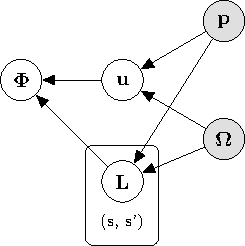
\includegraphics{graphical_models/pgm2.pdf}
\end{figure}

With the following analytical form:-
\begin{equation}
\begin{split}
P(\mathbf{\Phi}, \mathbf{\Omega}, \mathbf{p}, \mathbf{u}, \mathbf{L}) = 
P(\mathbf{\Phi}|\mathbf{u})
\prod_{(s, s') \in \mathcal{S}}P(\mathbf{u}|\mathbf{\Omega}, \mathbf{p}, \mathbf{L}_{(s, s')})\\
P(\mathbf{L}_{(s, s')}|\mathbf{\Omega}, \mathbf{p})
P(\mathbf{L}_{(s, s')})
\end{split}
\end{equation}

\subsection{Inferring Deformations}
The tracking consistency constraint denoted by the variable $\mathbf{L}$ in the above graphical model can be enforced in terms of minimising the 
transformations between adjacent submaps, such that the camera poses tracked in each subvolume are consistent. This follows the approach 
of\cite{Kahler2016}.  However, the approach proposed in this work differs in that the optimisation is integrated in to the probabilistic 
formulation previously outlined. Given instantaneously inferred transforms between subvolumes obtained from tracking results, 
the objective is to infer a robust, consistent deformation transformation for the subvolume pair.

As such, for each pair of visible subvolumes $(s, s')$, the following posterior must be maximised:-
\begin{equation}
\begin{split}
%Bayes rule + chain rule for P(omega, p)
P(\mathbf{\Omega}, \mathbf{p} | \mathbf{L}_{(s, s')}) = \frac{P(\mathbf{L}_{(s, s')} | \mathbf{\Omega}, \mathbf{p}) P(\mathbf{\Omega} | \mathbf{p})P(\mathbf{p})}
{P(\mathbf{L}_{(s, s')})}
\end{split}
\end{equation}
The intuition behind the above equation is that the deformation $\mathbf{L}_{(s, s')}$ applied to the probability field $\mathbf{u}$ should 
increase the probability of observing the current pose $\mathbf{p}$ given the current RGBD frame $\mathbf{\Omega}$ by reducing the 
variance of the camera tracking result. As such, global tracking variance is reduced by enforcing local consistency, improving the quality 
of the reconstruction.

The maximisation of the above posterior consists of a two stage process. Firstly, as a preprocessing step, the true transformation between 
subsegments is estimated over time from observed offsets, as documented in the following section. This inferred transformation is used to 
initialise a gradient based maximisation of the above posterior to yield an optimal deformation. The intuition behind this schema is that the 
gradient based optimisation routine is used to refine the inferred transformations between subsegments, improving robustness.

The following proportionality to the distribution over deformations is made:-
\begin{equation}
\begin{split}
P(\mathbf{L}_{(s, s')} | \mathbf{\Omega}, \mathbf{p}) \propto P(F_{s}(\mathbf{x}) | F_{s'}(G(\mathbf{x})))
\end{split}
\end{equation}
With the likelihood function taking the following form(a Gaussian distribution is assumed):-
\begin{equation}
\begin{split}
P(F_{s'}(G(\mathbf{x}))) = \prod_{(s, s') \in \mathcal{S}} \frac{1}{\sqrt{2 \pi \sigma}} \exp{\frac{-(F_{s}(\mathbf{x}) - F_{s'}(G(\mathbf{x})))^2}{2\sigma^2}}
\end{split}
\end{equation}
Or alternatively:-
\begin{equation}
\begin{split}
\ln P(F_{s'}(G(\mathbf{x}))) = m\ln\frac{1}{\sqrt{2\pi}\sigma}\\
-\frac{1}{2\sigma^2} \sum_{(s, s') \in \mathcal{S}} \bigg( F_{s}(\mathbf{x}) - F_{s'}(G(\mathbf{x})) \bigg)^2
\end{split}
\end{equation}
Where $F(.)$ is a scalar valued SDF(Signed Distance Function), $\mathbf{x}$ is a point represented by a 3-vector, and $G(.)$ is a transformation function taking
the following form:-
\begin{equation}
\begin{split}
G(\mathbf{x}) = \mathbf{R}(r_{1}, r_{2}, r_{3})\mathbf{x} + \mathbf{t}
\end{split}
\end{equation}
Where $\mathbf{R}(.)$ is a rotation matrix from the Special Orthogonal group $\mathbbm{SO}(3)$ paramaterised by the three Modified 
Rodrigues Parameters\cite{Shuster1993} $r_{1}$, $r_{2}$ and $r_{3}$.

Note that the logarithmic form of the above likelihood is suitable to Nonlinear Least Squares optimisation, allowing the posterior of equation 4 
to be maximised in terms of the likelihood term of equation 4. To perform MLE(Maximum Likelihood Estimation) over this likelihood using 
an optimisation routine such as Levenberg Marquardt, the following gradients must be computed for the rotational component of the 
deformation:-
\begin{equation}
\begin{split}
\frac{\partial E}{\partial r_{n}} = \frac{\partial E}{\partial F} \frac{\partial F}{\partial G} \frac{\partial G}{\partial r_{n}} \text{for } n \in {1,2,3}
\end{split}
\end{equation}
Similarly for the translational component:-
\begin{equation}
\begin{split}
\frac{\partial E}{\partial \mathbf{t}_{d}} = \frac{\partial E}{\partial F} \frac{\partial F}{\partial G} \frac{\partial G}{\partial \mathbf{t}_{d}} \text{for } d \in {x,y,z}
\end{split}
\end{equation}

\subsection{Estimation of Inter-Subvolume Constraints}
Due to the on-line nature of the fusion pipeline there is a degree of uncertainty around the measured offsets between subvolumes. As such, to 
counter this and yield a robust starting constraint for the previously described optimisation procedure, a recursive bayesian estimation 
procedure is used to estimate the true pose difference between two subvolumes.

As such, the update for the starting deformation transformation $\mathbf{L}_{t}$ may be defined in 
terms of $\mathbf{L}_{t-1}$ and observed offsets transforms between segments $\mathbf{Z_{(s, s')}} = \mathbf{T}_{s}^{-1}\mathbf{T}_{s'}$  in a predict-update fashion, using the following prediction equation:-
\begin{equation}
\begin{split}
P(\mathbf{L}_{i} | \mathbf{Z}_{1:i-1}) = \int P(\mathbf{L}_{i} | \mathbf{L}_{i-1})P(\mathbf{L}_{i-1} | \mathbf{Z}_{1:i-1}) d\mathbf{L}_{i-1}
\end{split}
\end{equation}
and update equation
\begin{equation}
\begin{split}
P(\mathbf{L}_{i} | \mathbf{Z}_{1:i}) = \frac{P(\mathbf{Z}_{i} | \mathbf{L}_{i})P(\mathbf{L}_{i} | \mathbf{Z}_{1:i-1})}{P(\mathbf{Z}_{i} | \mathbf{Z}_{1:i-1})}
\end{split}
\end{equation}
where
\begin{equation}
\begin{split}
P(\mathbf{Z}_{i} | \mathbf{Z}_{1:i-1}) = \int P(\mathbf{Z}_{i} | \mathbf{L}_{i})P(\mathbf{L}_{i} | \mathbf{Z}_{1:i-1}) d\mathbf{L}_{i}
\end{split}
\end{equation}
However, it should be noted that the denominator of the update equation may in practice be replaced with a normalisation constant as follows:-
\begin{equation}
\begin{split}
P(\mathbf{L}_{i} | \mathbf{Z}_{1:i}) = \alpha P(\mathbf{Z}_{i} | \mathbf{L}_{i})P(\mathbf{L}_{i} | \mathbf{Z}_{1:i-1})
\end{split}
\end{equation}
Note that in the above equations, the constraint pair subscript has been dropped for clarity in notation.

This online prediction-update schema will allow the evolution of pose difference constraints over time increasing their robustness at the time 
of optimisation of deformations.